\documentclass[tikz,border=6pt]{standalone}
% ============================================================================
%  VeriGate diagram design system (shared by every standalone figure).
%  Goals: bold, legible, print-safe; shape carries notation, colour reinforces
%  outcome; arrow labels sit on tinted pills so they never erase the arrow line;
%  no mid-word hyphenation inside nodes.
% ============================================================================
\usepackage[T1]{fontenc}
\usepackage{fouriernc}
\usetikzlibrary{arrows.meta,positioning,calc,fit,shapes.geometric,shapes.symbols,shapes.misc,backgrounds,shadows.blur}

% --- Never hyphenate words inside nodes (the main "sloppy / AI" tell) ---
\hyphenpenalty=10000
\exhyphenpenalty=10000
\tolerance=2000
\hbadness=10000

% --- Palette: cohesive, saturated enough to read, safe in grayscale ---
\definecolor{vgNavy}{HTML}{1F4E79}   % processes / primary
\definecolor{vgTeal}{HTML}{0E7C86}   % success / interaction
\definecolor{vgAmber}{HTML}{C8841B}  % decisions
\definecolor{vgSlate}{HTML}{4C5A68}  % external entities / stores
\definecolor{vgRed}{HTML}{C0453B}    % errors / reject / deny
\definecolor{vgGreen}{HTML}{2E8B57}  % final success outcome
\definecolor{vgViolet}{HTML}{6A4C93} % highlight / novel step
\definecolor{vgInk}{HTML}{2A3440}    % arrows & strokes
\definecolor{vgPaper}{HTML}{F4F1EA}  % label-pill background

\tikzset{
  % ---------- shared helpers ----------
  vgshadow/.style={blur shadow={shadow blur steps=5,shadow xshift=0.5pt,
      shadow yshift=-0.7pt,shadow opacity=28,shadow blur radius=1.4pt}},
  >={Stealth[length=2.6mm,width=2.1mm]},
  % ---------- data-flow (Yourdon/DeMarco) ----------
  dfdprocess/.style={circle,draw=vgNavy,line width=1.1pt,fill=vgNavy!14,
    align=center,font=\large\bfseries,text width=2.55cm,minimum size=3.15cm,
    inner sep=2pt,vgshadow},
  dfdentity/.style={rectangle,rounded corners=2pt,draw=vgSlate,line width=1pt,
    fill=vgSlate!14,align=center,font=\large,text width=2.6cm,minimum height=1.25cm,
    inner sep=5pt,vgshadow},
  dfdstore/.style={draw=none,align=center,font=\large,text width=3.1cm,
    minimum height=1.05cm,inner sep=4pt,
    append after command={\pgfextra{%
      \fill[vgTeal!8] (\tikzlastnode.north west) rectangle (\tikzlastnode.south east);
      \draw[vgSlate,line width=1pt]
        (\tikzlastnode.north west)--(\tikzlastnode.north east)
        (\tikzlastnode.south west)--(\tikzlastnode.south east);
      \draw[vgSlate,line width=1pt]
        ([xshift=5mm]\tikzlastnode.north west)--([xshift=5mm]\tikzlastnode.south west);}}},
  dfdflow/.style={-{Stealth[length=2.6mm,width=2.1mm]},line width=1pt,draw=vgInk,
    rounded corners=2pt},
  dfdlabel/.style={font=\normalsize,align=center,fill=vgPaper,draw=vgSlate!45,
    line width=0.3pt,rounded corners=2pt,inner sep=2.6pt},
  % ---------- flowcharts ----------
  fcstart/.style={rounded rectangle,draw=vgTeal,line width=1.1pt,fill=vgTeal!16,
    align=center,font=\normalsize\bfseries,text=vgInk,minimum height=10mm,
    inner sep=5pt,vgshadow},
  fcgo/.style={fcstart,draw=vgGreen,fill=vgGreen!16},           % final success
  fcerror/.style={fcstart,draw=vgRed,fill=vgRed!14},            % error / deny exit
  fcstep/.style={rectangle,rounded corners=3.5pt,draw=vgNavy,line width=1pt,
    fill=vgNavy!12,align=center,font=\normalsize,text=vgInk,text width=3.6cm,
    minimum height=11mm,inner sep=5pt,vgshadow},
  fckey/.style={fcstep,draw=vgViolet,line width=1.3pt,fill=vgViolet!14,
    font=\normalsize\bfseries},                                 % highlighted step
  fcdecision/.style={diamond,aspect=2.1,draw=vgAmber,line width=1.1pt,
    fill=vgAmber!22,align=center,font=\normalsize\bfseries,text=vgInk,
    text width=2.7cm,inner sep=1pt,vgshadow},
  fcarrow/.style={-{Stealth[length=2.6mm,width=2.1mm]},line width=1pt,draw=vgInk,
    rounded corners=3pt},
  fclabel/.style={font=\small\bfseries,fill=vgPaper,draw=vgSlate!45,line width=0.3pt,
    rounded corners=2pt,inner sep=2.4pt,align=center},
  fcyes/.style={fclabel,text=vgGreen,draw=vgGreen!50},
  fcno/.style={fclabel,text=vgRed,draw=vgRed!50},
  % ---------- sequence (kept for compatibility) ----------
  sqhead/.style={rectangle,rounded corners=2pt,draw=vgNavy,line width=1pt,
    fill=vgNavy!14,align=center,font=\normalsize\bfseries,minimum height=9mm,
    text width=2.3cm,inner sep=2pt,vgshadow},
  sqlife/.style={densely dashed,draw=vgSlate!60,line width=.6pt},
  sqcall/.style={-{Stealth[length=2.6mm]},line width=1pt,draw=vgInk},
  sqreply/.style={-{Stealth[length=2.6mm]},dashed,line width=.8pt,draw=vgInk},
  sqlabel/.style={font=\small,fill=vgPaper,draw=vgSlate!45,line width=.3pt,
    rounded corners=2pt,inner sep=2.2pt},
  sqframe/.style={draw=vgSlate,line width=.8pt,fill=white},
  sqtag/.style={font=\small,anchor=north west,draw=vgSlate,fill=vgTeal!18,inner sep=2pt},
  % ---------- deployment / components ----------
  component/.style={rectangle,rounded corners=3pt,draw=vgNavy,line width=1pt,
    fill=vgNavy!12,align=center,font=\normalsize,text=vgInk,minimum height=11mm,
    inner sep=6pt,vgshadow},
  comphi/.style={component,draw=vgTeal,line width=1.2pt,fill=vgTeal!14},
  boundary/.style={rectangle,rounded corners=4pt,draw=vgSlate,line width=1pt,
    fill=vgSlate!6,inner sep=3pt},
  link/.style={-{Stealth[length=2.6mm,width=2.1mm]},line width=1pt,draw=vgInk,
    rounded corners=2pt},
  linklabel/.style={font=\small\bfseries,fill=vgPaper,draw=vgSlate!45,line width=.3pt,
    rounded corners=2pt,inner sep=2.4pt,align=center},
  statelabel/.style={rectangle,rounded corners=3pt,draw=vgNavy,line width=1pt,
    fill=vgNavy!14,align=center,font=\normalsize,minimum height=10mm,inner sep=5pt,vgshadow}
}

\begin{document}
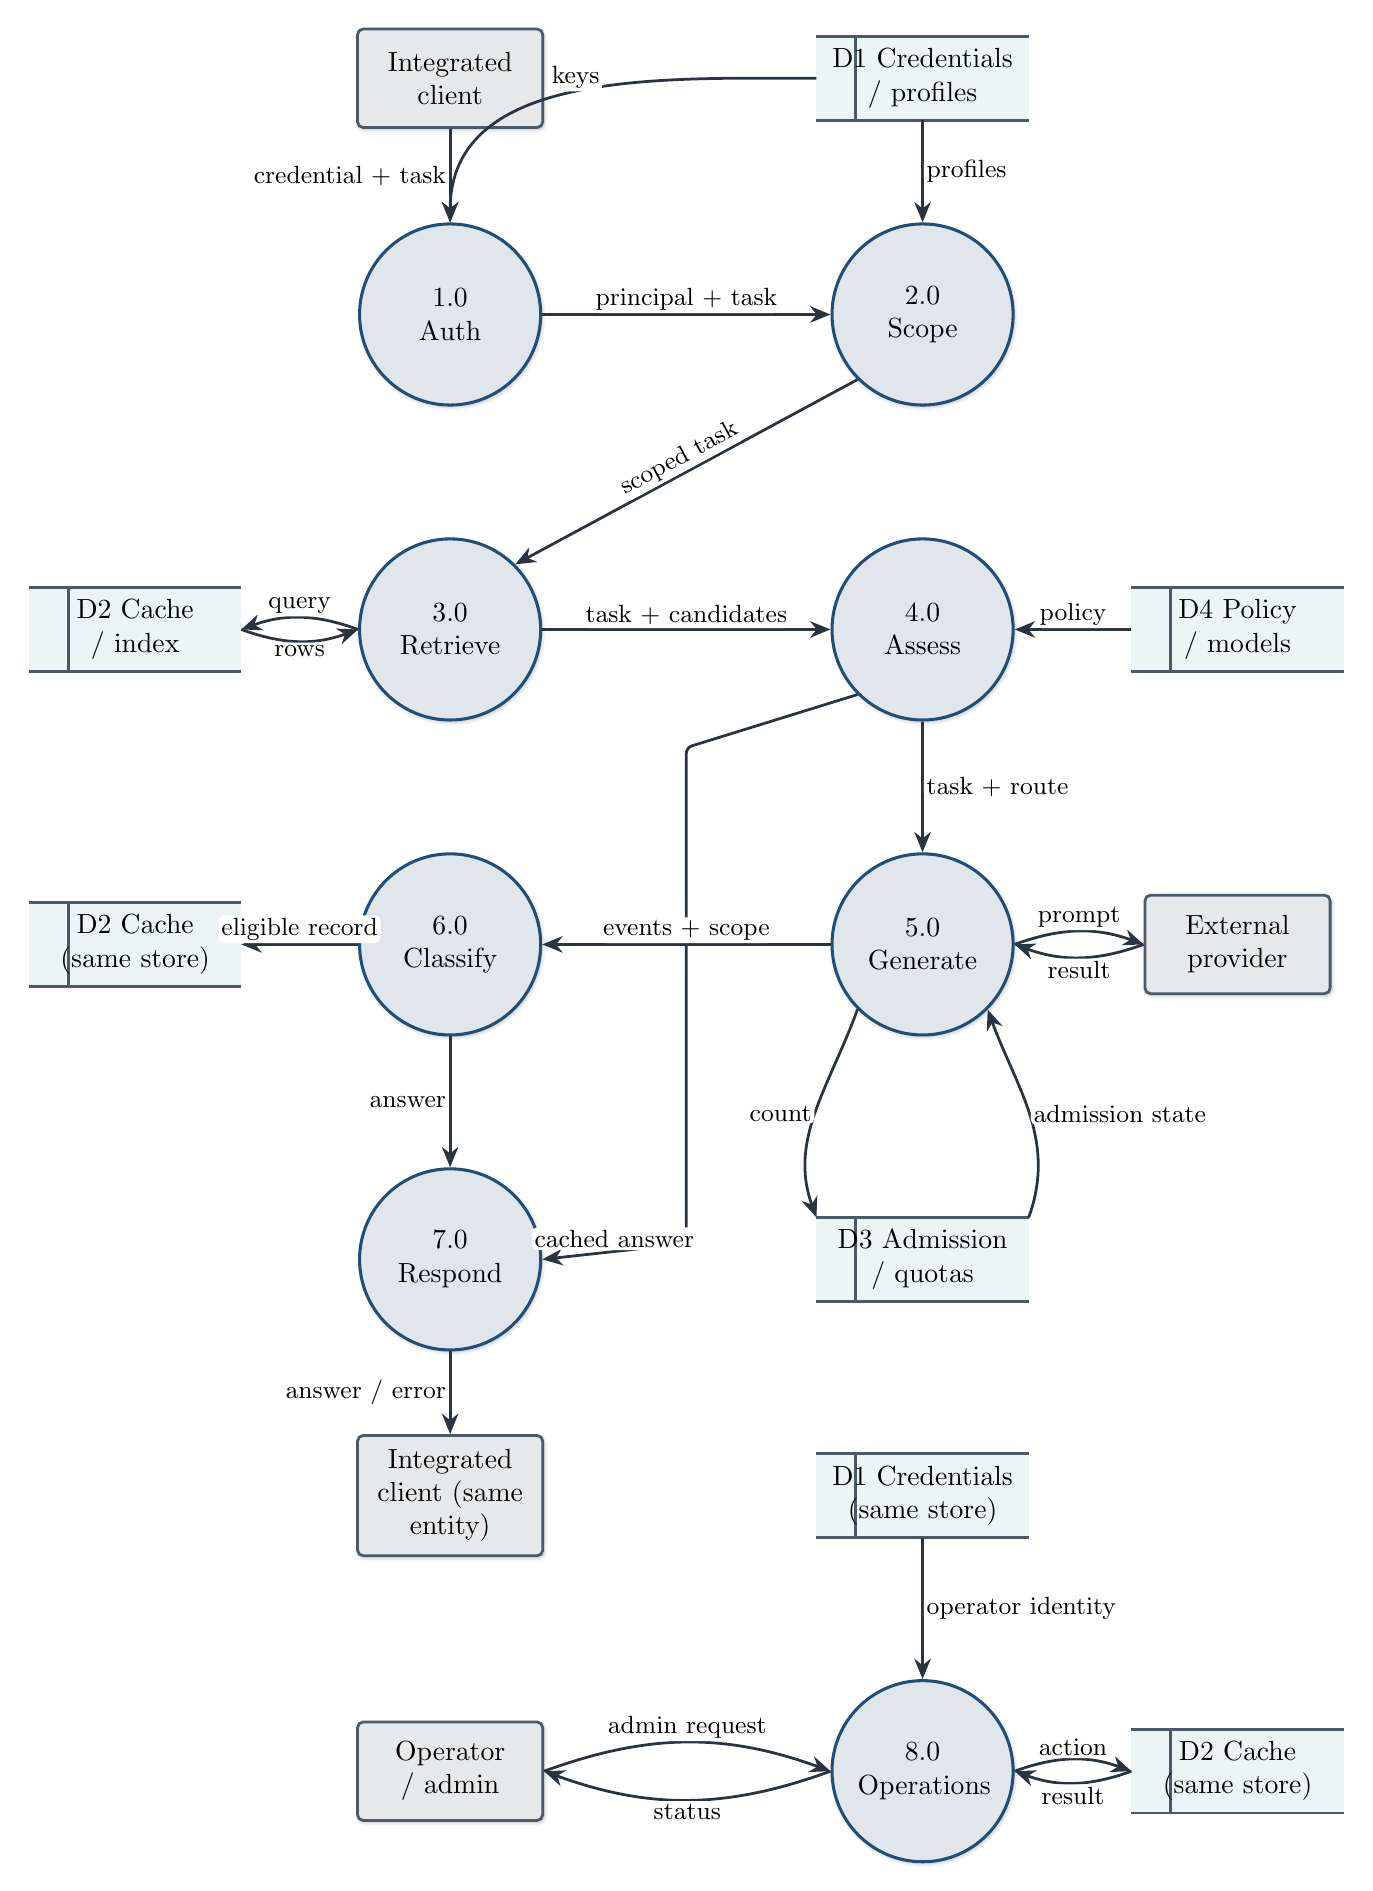
\begin{tikzpicture}

\tikzset{bubble/.style={dfdprocess,text width=1.65cm,minimum size=2.3cm,font=\normalsize},ext/.style={dfdentity,text width=2cm,font=\normalsize},store/.style={dfdstore,text width=2.4cm,font=\normalsize},lab/.style={font=\small,fill=white,align=center,inner sep=1pt}}
\node[ext] (client) at (0,0) {Integrated client};
\node[bubble] (p1) at (0,-3) {1.0\\Auth};
\node[bubble] (p2) at (6,-3) {2.0\\Scope};
\node[store] (d1) at (6,0) {D1 Credentials / profiles};
\node[bubble] (p3) at (0,-7) {3.0\\Retrieve};
\node[bubble] (p4) at (6,-7) {4.0\\Assess};
\node[store] (d2) at (-4,-7) {D2 Cache / index};
\node[store] (d4) at (10,-7) {D4 Policy / models};
\node[bubble] (p5) at (6,-11) {5.0\\Generate};
\node[ext] (provider) at (10,-11) {External provider};
\node[store] (d3) at (6,-15) {D3 Admission / quotas};
\node[bubble] (p6) at (0,-11) {6.0\\Classify};
\node[store] (d2w) at (-4,-11) {D2 Cache (same store)};
\node[bubble] (p7) at (0,-15) {7.0\\Respond};
\node[ext] (client2) at (0,-18) {Integrated client (same entity)};
\node[ext] (admin) at (0,-21.5) {Operator / admin};
\node[bubble] (p8) at (6,-21.5) {8.0\\Operations};
\node[store] (d1a) at (6,-18) {D1 Credentials (same store)};
\node[store] (d2a) at (10,-21.5) {D2 Cache (same store)};
\draw[dfdflow] (client)--node[lab,left]{credential + task}(p1);
\draw[dfdflow] (d1.west) to[out=180,in=90] node[lab,above]{keys}(p1.north);
\draw[dfdflow] (d1)--node[lab,right]{profiles}(p2);
\draw[dfdflow] (p1)--node[lab,above]{principal + task}(p2);
\draw[dfdflow] (p2.south west)--node[lab,above,sloped]{scoped task}(p3.north east);
\draw[dfdflow] (p3.west) to[out=160,in=20] node[lab,above]{query}(d2.east);
\draw[dfdflow] (d2.east) to[out=340,in=200] node[lab,below]{rows}(p3.west);
\draw[dfdflow] (p3)--node[lab,above]{task + candidates}(p4);
\draw[dfdflow] (d4)--node[lab,above]{policy}(p4);
\draw[dfdflow] (p4)--node[lab,right]{task + route}(p5);
\draw[dfdflow] (p4.south west)--(3,-8.5)--(3,-14.8)--node[lab,above]{cached answer}(p7.east);
\draw[dfdflow] (p5.east) to[out=20,in=160] node[lab,above]{prompt}(provider.west);
\draw[dfdflow] (provider.west) to[out=200,in=340] node[lab,below]{result}(p5.east);
\draw[dfdflow] (p5)--node[lab,above]{events + scope}(p6);
\draw[dfdflow] (p5.south west) to[out=250,in=110] node[lab,left]{count}(d3.north west);
\draw[dfdflow] (d3.north east) to[out=70,in=290] node[lab,right]{admission state}(p5.south east);
\draw[dfdflow] (p6)--node[lab,above]{eligible record}(d2w);
\draw[dfdflow] (p6)--node[lab,left]{answer}(p7);
\draw[dfdflow] (p7)--node[lab,left]{answer / error}(client2);
\draw[dfdflow] (admin.east) to[out=20,in=160] node[lab,above]{admin request}(p8.west);
\draw[dfdflow] (p8.west) to[out=200,in=340] node[lab,below]{status}(admin.east);
\draw[dfdflow] (d1a)--node[lab,right]{operator identity}(p8);
\draw[dfdflow] (p8.east) to[out=20,in=160] node[lab,above]{action}(d2a.west);
\draw[dfdflow] (d2a.west) to[out=200,in=340] node[lab,below]{result}(p8.east);

\end{tikzpicture}
\end{document}
